\chapter{Related Studies }
In this chapter, priciples and theories utilized in this thesis will be introduced.


% ------------------------------------------------------------ %
\section{Research Methodology}
In the methodology section, the we first delves into the existing literature, drawing from a paper accessible through the platform "Paper with Code." This platform typically provides research papers along with their associated code implementations. The chosen paper appears to be selected based on its prominence, likely measured by its reported accuracy or success in the field.
Following the identification of the primary paper, the researcher conducts a thorough review of its content, focusing particularly on aspects related to methodology. This involves understanding the proposed techniques, algorithms, and approaches presented in the paper to achieve high accuracy in the context of text-based person searches. The aim is to comprehend the nuances of the existing methodology and identify the key factors contributing to its success.
In addition to the primary paper, the researcher examines two other papers that exhibit a significant difference in accuracy. This comparative analysis is valuable for gaining insights into different approaches within the field. The choice of these additional papers may be strategic, aiming to capture diverse perspectives or methodologies, especially if there is a notable contrast in their reported accuracy metrics.
The researcher likely scrutinizes the methodologies of these selected papers, comparing and contrasting them with the primary paper. This comparative analysis helps identify the strengths and weaknesses of different approaches, shedding light on potential areas of improvement or innovation for the current research.
Overall, the methodology involves a comprehensive exploration of relevant literature, with a focus on the primary paper selected from "Paper with Code." The intent is to understand the methodologies employed in achieving high accuracies and to leverage insights from other papers with varying performance metrics. 

However, if only paperwithcode is used, the information obtained is limited and biased. To eliminate this bias, we decided to use scopus to search a wider range of papers by keyword search.

\subsection*{Identification}

The following research question was defined:

\bigskip
\textit{``How does the model compares with the text information with the image information''}
\bigskip



From this research question, four main keywords that sufficiently explain the topic were used: person retrieval and vision language pre-training.
Furthermore, synonyms and related terms were associated to these keywords to form keyword groups as follows:

\begin{itemize}
    \item person retrieval:
    \begin{itemize}
        \item person;
        \item person detection;
        \item person search.
    \end{itemize}
    \item vision language pre-training:
    \begin{itemize}
        \item VLP;
        \item text based;
        \item text.
    \end{itemize}
\end{itemize}


From the keywords, we had a keyword search on scopus from the search strings as follows:

\begin{itemize}
    \item ( "person retrieval" OR "person" OR "person detection" OR "person search" ) AND ( "vision language pre-training" OR "VLP" OR "text based" OR "text" ).
\end{itemize}

The Scopus search yielded a total of $20170$ documents. Within this result, we set the subject area to Computer Science, document type to article and conference paper, language to only english, and set the open access to all open access. With this filters, $862$ articles were found. 

\subsection{Screening}

Various factors were taken into account for the exclusion of documents:
\begin{enumerate}
    \item problem and goal were too different (e.g., building new hardware, analysis of leaf reflectance);
    \item not sufficiently related to this work (e.g., focused on hyperspectral );
    \item duplicates that were not automatically detected and excluded.
\end{enumerate}

% ------------------------------------------------------------ %

\section{Vision-language models}
Vision-language model have been researched significantly by leveraging end-to-end trainable deep neural networks (DNN). Before the vision-language model, both vision and language were researched with different DNN model structures. 

Vision recognition research have been updated until recent studies. Until now, the vision recognition models have experienced 5 stages, including traditional machine learning, deep learning from scratch, supervised pre-training with fine-tuning, unsupervised pre-training with fine-tuning, and vision-language model with pre-training.

Traditional machine learning relied on feature engineering. To achieve features, general methods were to hand-craft features \cite{svmclassification} and lightweight models \cite{knn}\cite{svm} to classify images into predefined categories. However, this method demands domain experts to design effective features for specific visual recognition tasks, which makes it ineffective for complex tasks and limits its scalability.

To overcome the problems with traditional methods, deep learning methods were devised \cite{imagenet} \cite{dnn_imagerecognition} to enhance the feature engineering and allowed to focus on the architecture engineering of neural networks to learn features effectively.
Great success from ResNet \cite{resnet}, which is a deep learning model introducing residual connections as a solution to the gradient vanishing problem.

1. Traditional Machine Learning and Prediction
Early visual recognition relied on hand-crafted features and lightweight models to classify images into predefined categories.
This method required domain experts and struggled with complex tasks and scalability.
2. Deep Learning from Scratch and Prediction
With the advent of deep learning, visual recognition shifted to end-to-end trainable Deep Neural Networks (DNNs), removing the need for hand-crafted features.
Models like ResNet demonstrated the ability to train on large datasets, achieving unprecedented performance.
However, this approach faced issues such as slow training convergence and the need for extensive labeled data.
3. Supervised Pre-training, Fine-tuning, and Prediction
This paradigm pre-trains DNNs on large labeled datasets and then fine-tunes them on specific tasks.
It accelerates convergence and improves performance even with limited task-specific data by leveraging pre-learned visual knowledge.
4. Unsupervised Pre-training, Fine-tuning, and Prediction
To overcome the dependency on labeled data, this method uses self-supervised learning for pre-training on unlabeled data.
Techniques like masked image modeling and contrastive learning enable the model to learn transferable features.
This paradigm allows the use of more extensive data, often leading to better performance than supervised pre-training.
5. Vision-Language Model (VLM) Pre-training and Zero-shot Prediction
Inspired by natural language processing, this new approach pre-trains models using large-scale image-text pairs available on the internet.
These models, trained with vision-language objectives, can make zero-shot predictions on new tasks without additional fine-tuning.
This paradigm leverages vast amounts of web data, enabling effective and efficient visual recognition.


Vision-Language models are a model that combines both the vision and language modalities and enables to process both information. 
Take, for example, the task of zero-shot image classification. We’ll pass an image and a few prompts like so to obtain the most probable prompt for the input image.
To predict the probable prompt, the model needs to understand both input image and the text prompts. To understand those modalities, the model will have separate or fused encoders for both vision and language.


\subsection{Learning Strategies}
Contrastive learning aims to map input images and texts to the same feature space such that the distance between the embeddings of image-text pairs is minimized if they match or maximized if they don’t. This method is a commonly used pre-training objectives for vision models and proven to be a highly effective for vision-language models as well. \cite{radford2021learning} uses this learning strategy with a cosine distance between the text and image embeddings. For pre-training methods requires large datasets to train, so most of the times, they use image and corresponding caption from the internet to train. This way, the model can train with large data, but in the other hand the image and caption sometimes does not correlate. To deal with this problem, ALIGN\cite{jia2021scaling} and DeCLIP\cite{li2022supervision} designed their own distance metrics.


\subsection{BERT}
aaa


\subsection{ALBEF}
Text encoder and image encoder are used to learn the representation in vision-and-language pre-training models (VLP). Most existing VLP models use multi-modal encoder to jointly model visual token (image feature) and word tokens (text features). This methods face challenges because the visual and word tokens are unaligned, making it difficult for the encoder to learn interactions between them. 
To tackle this challenge, the author first aligns image and text representations before fusing them through cross-modal attentions. 

\begin{figure}[htbp]
    \begin{center}
        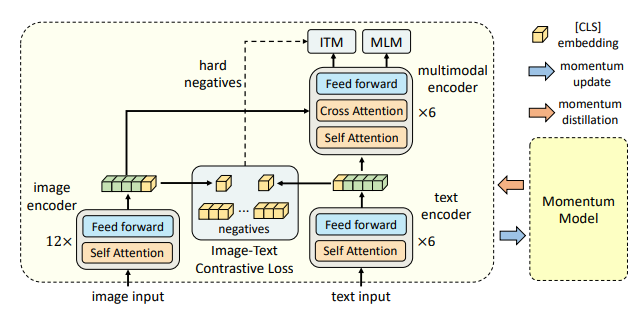
\includegraphics[width=10cm]{img/albef_model_structure.png}
        \caption{Structure of ALBEF}
        \label{fig:albef}
    \end{center}
\end{figure}

The author represented a model with an image encoder, text encoder, and a multi-modal encoder. They use 12-layer visual transformer ViT-B/16[\cite{dosovitskiy2021image}], pre-trained with ImageNet-1k, as the image encoder. 
Text encoder is pre-trained by the first 6 layers of $BERT_{base}$, and multi-modal encoder for fusing text and image features are pre-trained by the last 6 layers of $BERT_{base}$. The text encoder transform an input text $T$ into a sequence of embedding $\{w_{cls}, w_1, ..., w_N\}$. The image features also transform an input image $I$ into a sequence of embedding $\{v_{cls}, v_1, ..., v_M\}$. The text features are fed to a multi-modal encoder, while the image features are fused through cross attention at each layer of the multi-modal encoder.

Pretraining Objectives
The model have three objectives in pretraining: image-text contrastive learning (ITC) on the unimodal encoders, masked language modeling (MLM) and image-text matching (ITM).
Author utilizes the hard negative mined from ITC to improve ITM.

Image text contrastive learning is used to align the representation from the unimodal encoders before fusing. This objective makes it easier for the multi-modal encoder to perform cross-modal learning, as the input features are already aligned in a common space. 

Masked language modeling (MLM) is utilized with both image and text information to determine the masked text. Author randomly masks 15\% of the input token with specialized token [MASK]. The MLM minimizes the cross-entropy loss.

\begin{displaymath}
    L_{mlm} = \epsilon_{(I,\hat{T})~D}H(y^{msk}, p^{msk}(I,\hat{T}))
\end{displaymath}

$\hat{T}$ is masked text, $P^{msk}(I,\hat{T})$ is the model's predicted probability for a masked token. 

Contrastive loss is used for alignment, which helps to ground the vision and text representations.



\section{Person retrieval methods}
\subsection{RaSa}

Vision language models are very popular regions. Many studies have been published to be able to bind the visual information with the text information. Many methods have been proposed, but learning a powerful multimodal representation is still a challenging task. This author approches to this task by two innovations: Relation aware and Sensitivity aware.

The author remarked that the text and image pair of the same ID have a strong positive pair and weak positive pair. Since the textual discription is genereated by a single image in the text-based person search dataset, the text will strongly correlate to the image but it is not always well-aligned to the other images of the same person. Previous methods did not take this intra-variation into account when training, they put the equal weight for strong and weak positive pairs in learning representations. This lead the model to overfitting due to the weak pairs.

To reduce the impact of noise interference from weak positive pairs, the author introduced a Relation-Aware learning (RA) task. This task consists of a probabilistic Image-Text Matching (p-ITM) component and a Positive Relation Detection (PRD) component. The p-ITM is a variant of the commonly used ITM, designed to differentiate negative and positive pairs by probabilistically considering strong or weak positive inputs. Meanwhile, the PRD explicitly distinguishes between strong and weak positive pairs. In this framework, p-ITM focuses on the consistency between strong and weak positive pairs, whereas PRD emphasizes their differences, effectively acting as a regularization for p-ITM. By incorporating RA, the model can extract valuable information from weak positive pairs through p-ITM and reduce noise interference through PRD, ultimately achieving a balance.

Furthermore, improving the robustness of representations often involves learning invariant representations under a set of manually chosen transformations, referred to as insensitive transformations [Caron et al., 2020; Chen and He, 2021]. While this approach is recognized, we take it further by drawing inspiration from the recent success of equivariant contrastive learning [Dangovski et al., 2022]. We explore sensitive transformations that would degrade performance if applied to learn transformation-invariant representations. Instead of maintaining invariance under insensitive transformations, we encourage the learned representations to be aware of sensitive transformations. 

To achieve this, author proposed a Sensitivity-Aware learning (SA) task. They use word replacement as the sensitive transformation and develop a Momentum-based Replaced Token Detection (m-RTD) pretext task. This task involves detecting whether a token originates from the original textual description or the replacement, as illustrated in Figure 1 (b). The closer the replaced word is to the original one (i.e., the more confusing the word), the more challenging the detection task becomes. Training the model to effectively solve this detection task is expected to enhance its ability to learn better representations.

The author utilize Masked Language Modeling (MLM) to perform word replacement, leveraging the image and text contextual tokens to predict the masked tokens. Additionally, considering that a momentum model, which is a slow-moving average of the online model, can learn more stable representations than the current online model [Grill et al., 2020], author use MLM from the momentum model to generate more confusing words. 

Overall, MLM and m-RTD together form Sensitivity-Aware learning (SA), providing robust surrogate supervision for representation learning.


\section{Masking Strategies}
Methods for masking have many different varieties, so from those methods, I pick to change the masking ratio.